
\section{Experimental Analysis}\label{sec:exp}
These benchmarks were carried out on a Dell Mobile Precision Workstation 5760 with 
Intel Xeon W-11955M (8 Core, 24MB Cache, 2.60 GHz to 5.00 GHz, 45W, vPro), 64GB DDR4 3200MHz RAM and 400GB free disk space.
\begin{figure}[!t]
	\centering
%<<<<<<< HEAD
	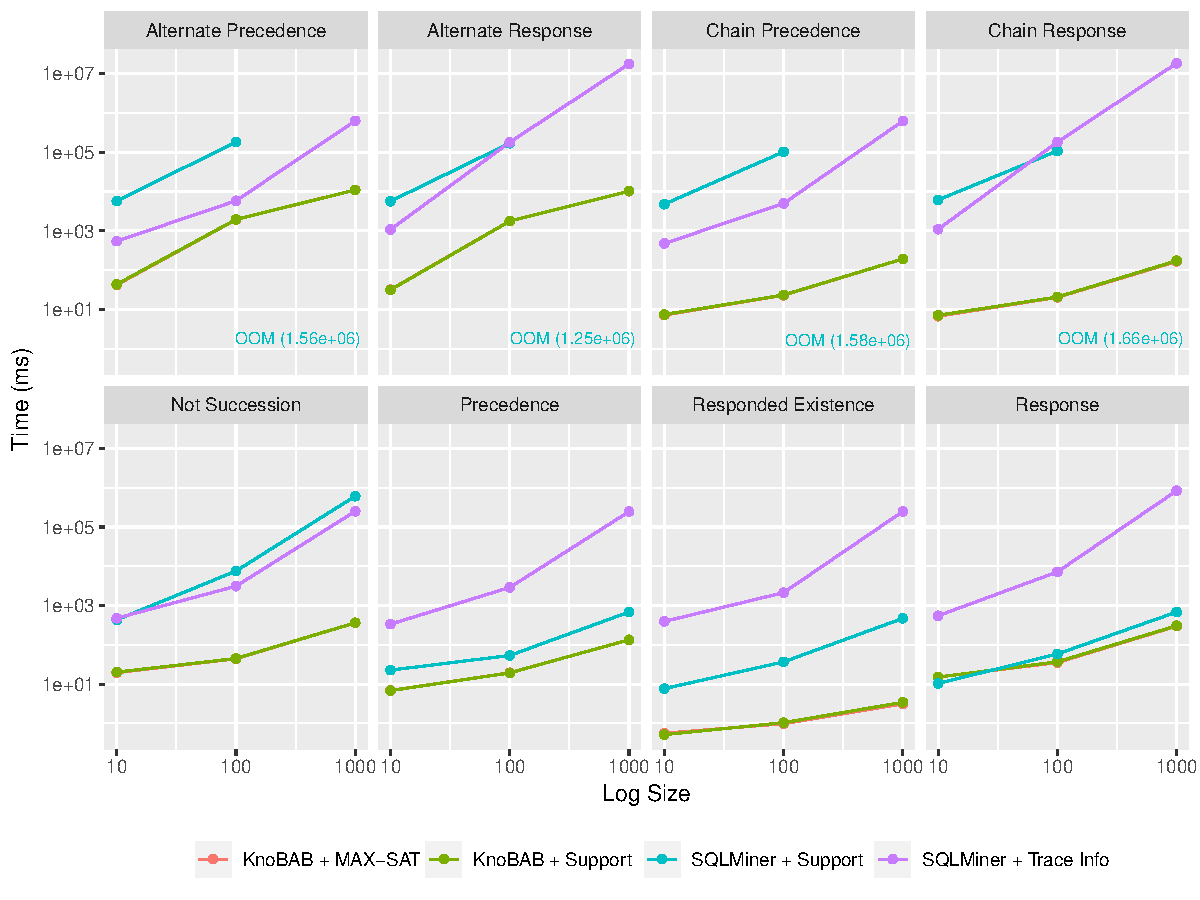
\includegraphics[width=.8\textwidth]{images/sqlminer_benchmark.pdf}
	\caption{KnoBAB vs SQLMiner Performance for 25  clauses with frequent activity labels with Support and Trace Information. OOM indicates Out of Primary Memory.}\label{fig:vsSQL}
%=======
%	\caption{KnoBAB vs SQLMiner Performance for Varying Model Size.}\label{fig:vsSQL}
%>>>>>>> 33357ef815c5a234b684fdafdceed45bf3a89be0
\end{figure}


\subsection{SQLMiner}\label{ssec:sqlmin}
These experiments want to test our working hypoteses related to the possibility to engineer a tailored relational database architecture outperforming process mining through conformance checking running on traditional relational databases, where no \LTLf operators are exploited and non-customary tabular representation is exploited. Given that the SQL provided in \cite{Schonig15,SchonigRCJM16} might only return the \textsc{Support} associated to each candidate declare clause (\texttt{SQLMiner+Support}), we provided the least possible changes to also associate to each candidate clause the set of all the traces satisfying it. By doing so, we extended the activation condition expressed in SQL and used \texttt{array\_aggr} provided by \textbf{PostgreSQL 13.6} to list such traces (\texttt{SQLMiner+TraceInfo}). For compare the same settings in KnoBAB, we run both Max-SAT and \textsc{Support} queries with the difference that, in our case, both of these implementations will always return per intermediate result specification the trace information satisfying each possible model clause.
We exploited the same hospital log dataset from \cite{SchonigRCJM16}. In order to test the scalability of the solutions, we tested the queries runtime with increasing log size: we randomly sampled the log with three sub-logs containing 10, 100 and 1000 traces, while guaranteeing that each sub-log is always a subset of the greater sub-logs. For each sub-log, we generated 8 distinct models, and each model contains 25 clauses instantiating the same declare template (\textit{elected template}) with different activation and target conditions. Those did not consider payload conditions, and were only considering the most frequent activity labels appearing in the sub-log. For SQLminer, each model was queried by running the SQL query corresponding to the \textit{elected template}, and the specific activation and target conditions from the model's clauses were specified as distinct rows in the \textsf{Action} table.

The outcome of such experiments is represented in \figurename~\ref{fig:vsSQL}, where each plot represents the running time associated to models containing the same \textit{elected template}. In the worst case scenario (\textsf{Response}), we exhibit similar query running times to SQLMiner run on PostgreSQL while, in the best case scenario, we outperform the relational database solution using SQL by at most 5 orders of magnitude. This is due to the fact that our query plan minimizes the access to the data queries and to the fact that our computation avoided explicit computations of aggregations by guaranteeing that the intermediate results are always sorted, and by performing counting operations via linear scans of the intermediate result representation. Our solution never exceeded the 64GB of primary memory while, for some queries, SQLMiner exceeded it, thus proving that our solution is also memory efficient. Our running times in the \textsf{RespExistence} plot are due to an efficient query plan only accessing the  \textsf{CountTable}, while the original SQL query had still to scan the whole \texttt{Log} table (similar to our \texttt{ActivityTable}), which contained all of the trace events. We also remind the reader that the \textsf{CountTable} can be efficiently created while scanning the whole log dataset. This further validates that an adequate tabular representation twinned with \xLTLf operators extending the \LTLf specification for tabular data provides a suitable solution. Last, running time of the Max-SAT problem and \textsc{Support} for KnoBAB exhibited similar running times, while in PostgreSQL those exhibit huge variations depending on the query-plan rewriting performed by PostgreSQL query engine. For some elected templates, our proposed \texttt{SQLMiner+TraceInfo} formulation proved also to be more efficient than the \texttt{SQLMiner+Support} queries originally proposed by \cite{Schonig15}.

\begin{figure}[!t]
	\centering
	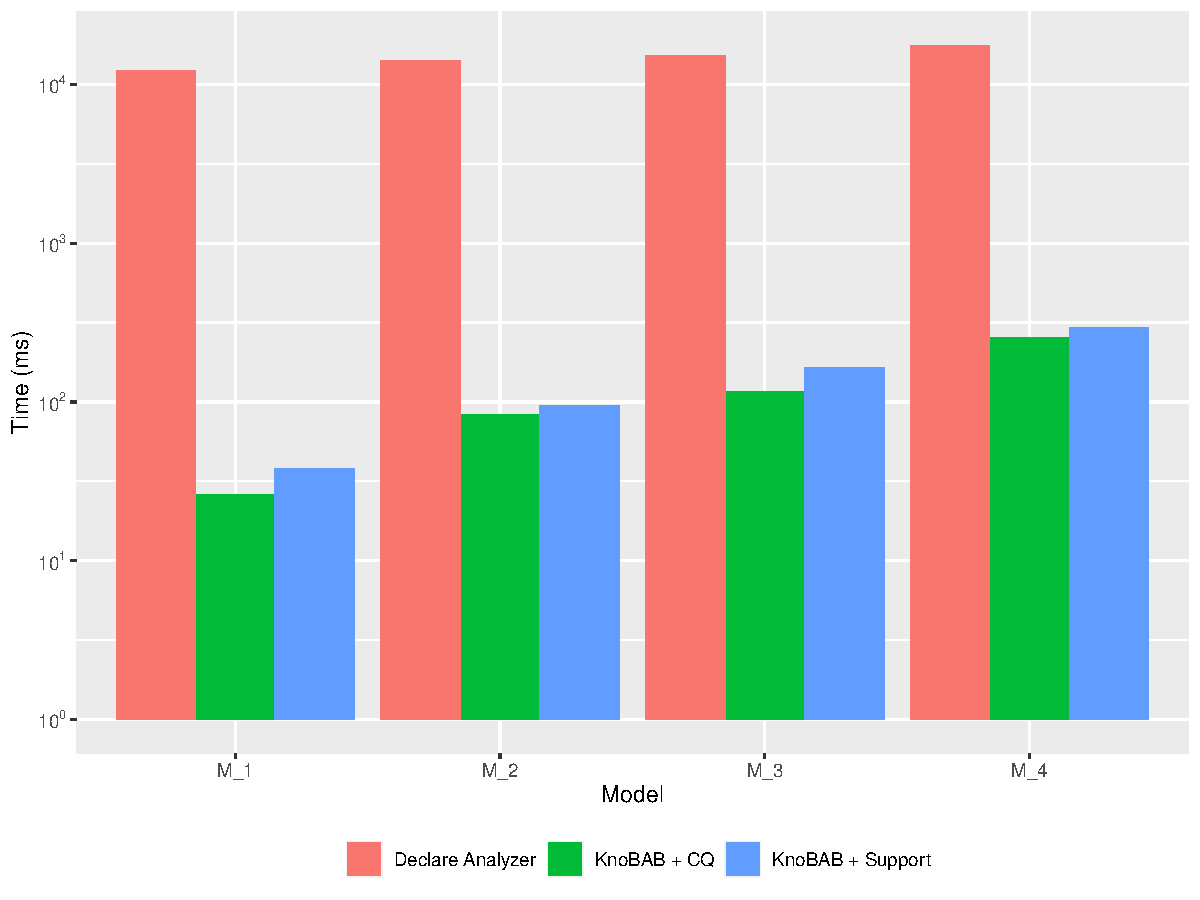
\includegraphics[width=.8\textwidth]{images/burattin_benchmark.pdf}
	\caption{KnoBAB vs Declare Analyzer Performance for Different Models.}\label{fig:vsSQL}
\end{figure}

%\subsection{Declare Analyzer}\label{ssec:declan}

%<<<<<<< HEAD
%\begin{figure}[!t]
%	\centering
%	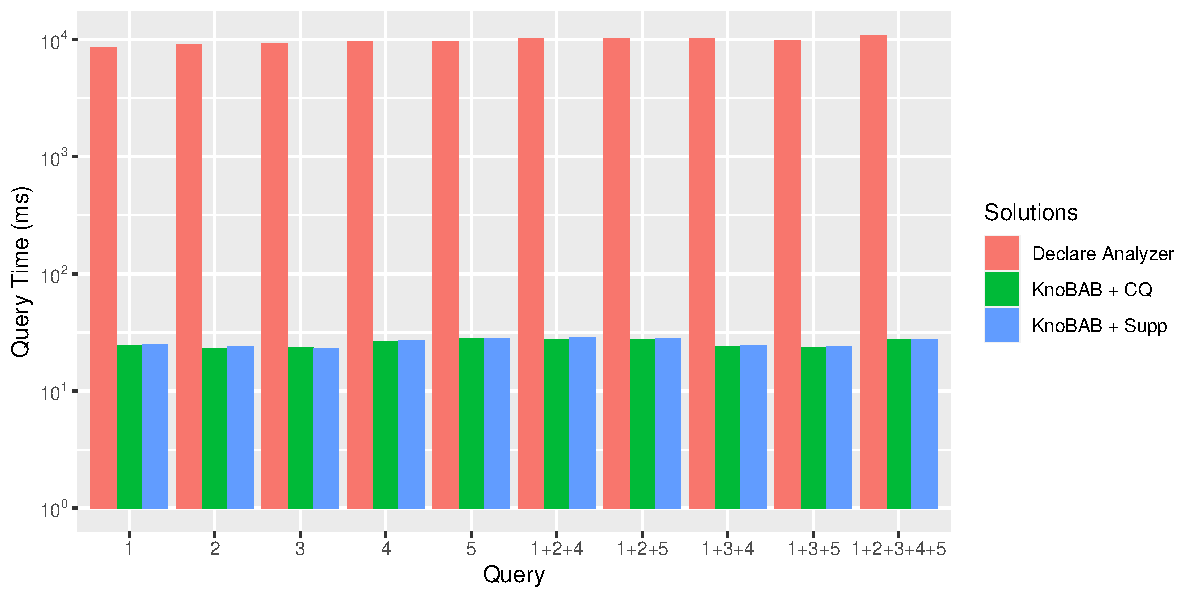
\includegraphics[width=.7\textwidth]{images/Buratto.pdf}
%	\begin{tabular}{l}
%		\toprule
%		\textit{Conjunctive Query}\\ 
%		\midrule
%		$q_1:= \DeclareClause{Response}{A\_SUBMITTED}{\textbf{true}}{A\_ACCEPTED}{\textbf{true}}$ \\
%		$q_2:= q_1\wedge \MonoDeclareClause{Exists}{\_\_trace\_payload}{\texttt{AMOUNT\_REQ}\geq 10^3}{\geq 1}$ \\
%		$q_3:=q_1\wedge \MonoDeclareClause{Exists}{\_\_trace\_payload}{\texttt{AMOUNT\_REQ}< 10^3}{\geq 1}$ \\
%		$q_4:=q_1\textrm{ where }\texttt{A\_SUBMITTED.org:resource}=\texttt{A\_ACCEPTED.org:resource}$ \\
%		$q_5:=q_1\textrm{ where }\texttt{A\_SUBMITTED.org:resource}\neq\texttt{A\_ACCEPTED.org:resource}$ \\
%		\bottomrule
%	\end{tabular}
%	\caption{KnoBAB vs Declare Analyzed Performance.}\label{fig:vsBuatto}
%\end{figure} 
\subsection{Declare Analyzer}\label{ssec:declan}
The set of experiments on Declare Analyzer have the aim of comparing our proposed solution against a solution tailored for solving Declare Conjunctive Queries over logs running exclusively in primary memory. In particular, we want to show the benefit of running a query plan when multiple sub-queries are shared: by increasing the size of the model by adding novel queries, we are expecting that while our solution exhibits a near constant running time, Declare Analyzer's running time should increase almost linearly as per the authors' claim.
%=======
\begin{table}[!t]
	\caption{Declare Models with their Respective Clauses}
	\resizebox{\textwidth}{!}{
		\begin{tabular}{l|l}
			Model & Queries \\
			\toprule
			\multirow{2}{*}{$M\_1=$} & $q_{1}:= \DeclareClause{Response}{A\_SUBMITTED}{\textbf{true}}{A\_ACCEPTED}{\textbf{true}}$ \\ & $q_{2}:= \DeclareClause{Response}{A\_SUBMITTED}{\texttt{AMOUNT\_REQ} \geq 10^3}{A\_ACCEPTED}{\textbf{true}}$ \\&
			$q_{3}:= \DeclareClause{Response}{A\_SUBMITTED}{\texttt{AMOUNT\_REQ} < 10^3}{A\_ACCEPTED}{\textbf{true}}$ \\&
			$q_{4}:= q_{1} \textrm{ where } \texttt{A\_SUBMITTED.org:resource}=\texttt{A\_ACCEPTED.org:resource}$ \\&
			$q_{5}:= q_{1} \textrm{ where } \texttt{A\_SUBMITTED.org:resource}\neq\texttt{A\_ACCEPTED.org:resource}$ \\
			\toprule
			\multirow{2}{*}{$M\_2=M_1+$} & $q_{6}:= \DeclareClause{Response}{W\_Completeren aanvraag}{\textbf{true}}{W\_Valideren aanvraag}{\textbf{true}}$ \\ &
			$q_{7}:= \DeclareClause{Response}{W\_Completeren aanvraag}{\textbf{true}}{O\_CANCELLED}{\textbf{true}}$ \\&
			$q_{8}:= q_{6} \textrm{ where } \texttt{A\_SUBMITTED.org:resource}\neq\texttt{A\_ACCEPTED.org:resource}$ \\&
			$q_{9}:= \DeclareClause{Response}{W\_Valideren aanvraag}{\texttt{AMOUNT\_REQ} = 5 \cdot 10^3}{O\_CANCELLED}{\textbf{true}} $ \\&
			$q_{10}:= q_{9} \textrm{ where } \texttt{A\_SUBMITTED.org:resource}=\texttt{A\_ACCEPTED.org:resource}$ \\
			\toprule
			\multirow{2}{*}{$M\_3=M_2+$} & $q_{11}:= \DeclareClause{Response}{O\_SELECTED}{\textbf{true}}{O\_CANCELLED}{\textbf{true}}$ \\&
			$q_{12}:= q_{11} \textrm{ where } \texttt{A\_SUBMITTED.org:resource}=\texttt{A\_ACCEPTED.org:resource}$ \\&
			$q_{13}:= \DeclareClause{Response}{O\_SELECTED}{\texttt{AMOUNT\_REQ} < 8 \cdot 10^3}{O\_CANCELLED}{\textbf{true}}$ \\&
			$q_{14}:= q_{13} \textrm{ where } \texttt{A\_SUBMITTED.org:resource}=\texttt{A\_ACCEPTED.org:resource}$ \\&
			$q_{15}:= \DeclareClause{Response}{O\_SELECTED}{\texttt{AMOUNT\_REQ} > 10^3}{O\_CANCELLED}{\textbf{true}}$ \\
			\toprule
			\multirow{2}{*}{$M\_4=M_3+$} & $q_{16}:= \DeclareClause{Response}{A\_PARTLYSUBMITTED}{\textbf{true}}{A\_DECLINED}{\textbf{true}}$ \\&
			$q_{17}:= q_{16} \textrm{ where } \texttt{A\_SUBMITTED.org:resource}=\texttt{A\_ACCEPTED.org:resource}$ \\&
			$q_{18}:= \DeclareClause{Response}{A\_PARTLYSUBMITTED}{\texttt{AMOUNT\_REQ} > 2 \cdot 10^4}{A\_DECLINED}{\textbf{true}}$ \\&
			$q_{19}:= \DeclareClause{Response}{A\_PARTLYSUBMITTED}{\texttt{AMOUNT\_REQ} > 2 \cdot 10^4}{A\_CANCELLED}{\textbf{true}}$ \\&
			$q_{20}:= q_{18} \textrm{ where } \texttt{A\_SUBMITTED.org:resource}=\texttt{A\_ACCEPTED.org:resource}$ \\
	\end{tabular}}
\end{table}

%>>>>>>> 33357ef815c5a234b684fdafdceed45bf3a89be0

In order to do so, we exploited the entire BPI 2012 Challenge dataset, also used in \cite{BurattinMS16}, and we slightly edited the queries in the same paper as illustrated in \figurename~\ref{fig:vsBuatto}. For Declare Analyzer, we choosed to load the dataset via MapDB\footnote{\url{https://mapdb.org/}}, thus aligning the authors' hash map representations of the dataset with a representation similar to the one for relational databases. 

Our experiments show that while our proposed solution has temporal fluctuations caused by the fact that the query was running on the order of the milliseconds, the running time for Declare Analyzer is constantly increasing with the number of the available queries. Overall, our solution outperforms by 2-3 orders of magnitude the one from Declare Analyzer.


%The benefits from the custom query plan are most obvious in the process mining stage, where a log consisting of potentially thousands of traces is tested against all combinations of clauses. However, computational gains can also be evidenced when the same querying approach is adapted to a runtime scenario, where we are querying only 1 trace against an existing model (which requires much less computation as a whole).
%
%For $\mathcal{C}$ Declare clauses, where $\mathcal{N}$ is the data loading cost, implementations without a KB suffer, resulting in $\mathcal{O(C \cdot N)}$ complexity. With a KB, data loading is necessary only once, enhancing the complexity to $\mathcal{O(C + N)}$.
%
%However these are computationally bottlenecked to the efficiency of these systems themselves, regardless of the optimality of the conformance checking.
%
%\RevDel{SQL miner, due to the query structure, requires vast amounts of secondary memory for temporary caching of query computation, {much less than KnoBAB requires}.}
